% Copyright 2004 by Till Tantau <tantau@users.sourceforge.net>.
%
% In principle, this file can be redistributed and/or modified under
% the terms of the GNU Public License, version 2.

% However, this file is supposed to be a template to be modified
% for your own needs. For this reason, if you use this file as a
% template and not specifically distribute it as part of a another
% package/program, I grant the extra permission to freely copy and
% modify this file as you see fit and even to delete this copyright
% notice. 

\documentclass{beamer}

% There are many different themes available for Beamer. A comprehensive
% list with examples is given here:
% http://deic.uab.es/~iblanes/beamer_gallery/index_by_theme.html
% You can uncomment the themes below if you would like to use a different
% one:
%\usetheme{AnnArbor}
%\usetheme{Antibes}
%\usetheme{Bergen}
%\usetheme{Berkeley}
%\usetheme{Berlin}
%\usetheme{Boadilla}
%\usetheme{boxes}
%\usetheme{CambridgeUS}
%\usetheme{Copenhagen}
%\usetheme{Darmstadt}
%\usetheme{default}
%\usetheme{Frankfurt}
%\usetheme{Goettingen}
%\usetheme{Hannover}
%\usetheme{Ilmenau}
%\usetheme{JuanLesPins}
%\usetheme{Luebeck}
\usetheme{Madrid}
%\usetheme{Malmoe}
%\usetheme{Marburg}
%\usetheme{Montpellier}
%\usetheme{PaloAlto}
%\usetheme{Pittsburgh}
%\usetheme{Rochester}
%\usetheme{Singapore}
%\usetheme{Szeged}
%\usetheme{Warsaw}

\usecolortheme{beaver}
\usepackage{listings}
\usepackage{minted}

\setbeamertemplate{itemize/enumerate body begin}{\Large}
\setbeamertemplate{itemize/enumerate subbody begin}{\large}

\newcommand{\shellcmd}[1]{\\\indent\indent\texttt{\footnotesize\# #1}\\}

\title{MIT-IIT Robotics Program}

% A subtitle is optional and this may be deleted
\subtitle{Getting Started, Compiling, Running, I/O, Variables, Expressions}

\author{Amartya Shankha Biswas}%\inst{1}}
% - Give the names in the same order as the appear in the paper.
% - Use the \inst{?} command only if the authors have different
%   affiliation.

% - Use the \inst command only if there are several affiliations.
% - Keep it simple, no one is interested in your street address.

\date{\today}
% - Either use conference name or its abbreviation.
% - Not really informative to the audience, more for people (including
%   yourself) who are reading the slides online

% Delete this, if you do not want the table of contents to pop up at
% the beginning of each subsection:
\AtBeginSubsection[]
{
  \begin{frame}<beamer>{Outline}
    \tableofcontents[currentsection,currentsubsection]
  \end{frame}
}

% Let's get started
\begin{document}

\begin{frame}
  \titlepage
\end{frame}

\begin{frame}{Outline}
  \tableofcontents`
  % You might wish to add the option [pausesections]
\end{frame}

% Section and subsections will appear in the presentation overview
% and table of contents.

\section{Introduction}

\begin{frame}{Instructors}{}
\begin{itemize}
	\item IIT Kharagpur
	\begin{itemize}
		\item Mayank Bhushan
		\item Sudarshan Sharma
		\item Manish Agarwal
		\item Sayan Sinha
		\item Mehul Nirala
		\item Rahul Kumar
	\end{itemize}
	\item MIT
	\begin{itemize}
		\item Amartya Shankha Biswas
		\item Maya Nasr
		\item Virup Gubba
	\end{itemize}
\end{itemize}
\end{frame}

\subsection{Curriculum}
\begin{frame}{C++ Basics}{}
\begin{itemize}
	\item Environment
	\begin{itemize}
		\item Ubuntu Linux
        \item Using the Terminal
        \item Compiling and Running C++ Code
	\end{itemize}
    \item Variables and Data Types
    \item Booleans, Comparison and Logic Flow
    \item Arrays and Loops
    \item Functions and Recursion
\end{itemize}
\end{frame}

\begin{frame}{Advanced C++}{Subject to change, based on feedback.}
\begin{block}{}
    We will decide which of these topics to teach, based on your feedback.
\end{block}
\begin{itemize}
    \item Graphics and Simulation
	\begin{itemize}
		\item 2D Graphics
        \item Physics Simulaton and Video Games
	\end{itemize}
	\item Object Oriented Programming
	\item Algorithms
	\begin{itemize}
		\item Searching
        \item Sorting
	\end{itemize}
	\item Standard Template Library
	\begin{itemize}
		\item Set
        \item Map
	\end{itemize}
\end{itemize}
\end{frame}

\begin{frame}{Microcontroller Programming}{Working with a tiny computer}
\begin{itemize}
	\item Control Theory (PID controller)
	\item Programming an Arduino
	\item Using a Resistive Touchscreen
	\item Driving Servo Motors
\end{itemize}
\end{frame}

\begin{frame}{Final Project}{Ball and Plate Balancing System}
\end{frame}


\section{Environment}

\subsection{Terminal and Basic Commands}
\begin{frame}{Terminal}
    \begin{block}{Opening Terminal}
        Open a terminal window by pressing \textbf{Ctrl+Alt+T}
    \end{block}
    \begin{figure}
        \centering
        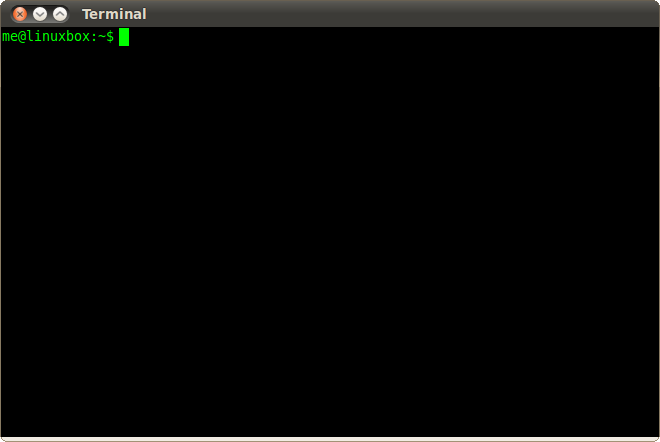
\includegraphics[width=\textwidth]{images/terminal.png}
    \end{figure}
\end{frame}

\begin{frame}{Directory Structure}
    \begin{figure}
        \centering
        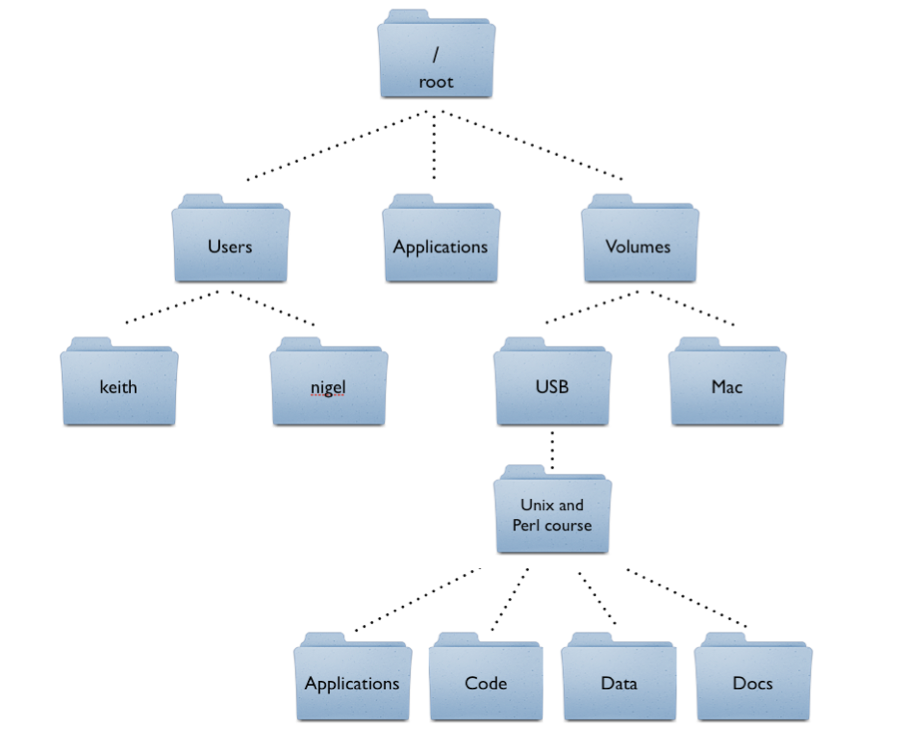
\includegraphics[height=0.7\textheight]{images/directory_tree.png}
    \end{figure}
\end{frame}

\begin{frame}[fragile]{Terminal Navigation}
    \begin{itemize}
        \item Make a new directory (folder)--
            \begin{minted}{bash}
                mkdir <directory_name>
            \end{minted}
        \item Enter a directory --
            \begin{minted}{bash}
                cd <directory_name>
            \end{minted}
        \item Type a command in the terminal, and then press \textbf{Enter}
    \end{itemize}
\end{frame}

\subsection{Editor}
\begin{frame}[fragile]{Text Editor}
    \begin{itemize}
        \item Write your code in a text editor
            \begin{itemize}
                \item Notepad, Vim, Emacs, etc.
            \end{itemize}
        \pause
        \item We will use \textbf{gedit}
        \pause
        \item Open \emph{gedit}
            \begin{minted}{bash}
                gedit &
            \end{minted}
        \item Open a file with \emph{gedit}
            \begin{minted}{bash}
                gedit my_file.cpp &
            \end{minted}
            \pause
            \begin{itemize}
                \item Note that the file should be present in your current directory
                \item If file doesn't exist, it will be created
            \end{itemize}
    \end{itemize}
\end{frame}


\section{Basics}

\section{Hello World}

\begin{frame}{Hello World !}{The First C++ Program}
  \inputminted{c++}{../code/hello_world/hello_world.cpp}
\end{frame}

\begin{frame}[fragile]{Compiling and Running}
  \begin{itemize}
      \item Use the following command to compile --
        \begin{minted}{bash}
            g++ -Wall hello_world.cpp
        \end{minted}
      \item This should create a file called \textbf{a.out} in your current directory.
      \item Use the following command to run the executable --
        \begin{minted}{bash}
            ./a.out
        \end{minted}
  \end{itemize}
\end{frame}

\subsection{Variables}

\begin{frame}{What is a Variable ?}{}
    \begin{block}{}
        A variable is a \textbf{name} that refers to a memory location.
    \end{block}
\end{frame}

\begin{frame}{Memory Location}{}
\end{frame}

\begin{frame}[fragile]{Data Types}{}

\begin{table}[]
\centering
\Large
\begin{tabular}{|l|l|l|}
\hline
\multicolumn{1}{|c|}{\textbf{Type}} & \multicolumn{1}{c|}
    {\textbf{Keyword}} & \multicolumn{1}{c|}{\textbf{Examples}} \\ \hline
Integer                  & int       & 0, -5, 43, 6             \\ \hline
Floating point           & float     & 2.5, -0.3, 0.0012, 1.0   \\ \hline
Double Floating point    & double    & 0.5, 9.1, -0.7, 7.0      \\ \hline
\end{tabular}
\end{table}
\end{frame}

\begin{frame}[fragile]{Variable Declaration}{}
    \begin{itemize}
        \item Variable contains Garbage Value (Un-initialized)
            \begin{minted}{c++}
                int a;
            \end{minted}
        \item Initializing with a value.
            \begin{minted}{c++}
                double b = 5.0;
            \end{minted}
        \item Declare multiple variables
            \begin{minted}{c++}
                int a, b, c, d;
            \end{minted}
    \end{itemize}
\end{frame}

\begin{frame}[fragile]{Variable Assignment}{NOT the same as ''equals''}
    \begin{block}{} Left side is name. Right side is value. \end{block}
    {
    \Huge \begin{minted}{c++}
        a = 5;
    \end{minted}
    \begin{minted}{c++}
        b = a + 5;
    \end{minted}
    }
    \begin{block}{} We \textbf{''assign''} a value to a variable. \end{block}
\end{frame}


\section{Expressions}

\begin{frame}{What is a Variable ?}{}
\end{frame}


\subsection{Comments}

\begin{frame}[fragile]{Comments}{Explaining what your code does}
    Anything following // will be ignored.
    \begin{block}{Single Line Comment}
        \begin{minted}{c++}
            a += 5; //Adding 5 to the value of a
        \end{minted}
    \end{block}
    Anything between /* and */ will be ignored.
    \begin{block}{Multi Line Comment}
        \begin{minted}{c++}
            int N = 0;
            /* This is a comment
            that spans
            multiple lines */
            cin >> N;
        \end{minted}
    \end{block}
\end{frame}


\subsection{Example}

\begin{frame}{Computing Squares}{Putting it All Together}
    \inputminted{c++}{../code/square/square.cpp}
\end{frame}

\begin{frame}{Computing Cubes}{}
    \inputminted{c++}{../code/cube/cube.cpp}
\end{frame}



\section{Exercises}

\begin{frame}[fragile]{Coding Practice}{}
    \begin{block}{Area of Circle}
        Write a program that takes as input the length of the radius of a circle, and outputs its area.
    \end{block}
    \begin{block}{Sum of First $N$ Natural Numbers}
        Write a program that takes as input an integer $N$, and computes the sum ($1+2+3+\cdots+N$).
        You may use the fact that $1+2+\cdots+N = \frac{N\cdot(N+1)}{2}$
    \end{block}
    \begin{block}{}
        Write a program that takes as input an integer $N$, and computes the sum
        of the last three digits of $N$.
        If there are less than three digits, just sum all of them.
    \end{block}
    \setbeamercolor{block title}{use=structure,fg=white,bg=red!35!black}
    \begin{block}{If you are familiar with C/C++}
        Write a program that takes as input an integer $N$, and computes the following sum.\\
        $\frac{6}{1^2}+\frac{6}{2^2}+\frac{6}{3^2}+\frac{6}{4^2}+\cdots+\frac{6}{N^2}$
    \end{block}
\end{frame}



\end{document}


